\documentclass[style=upen, size=14pt]{powerdot}
\definecolor{arany}{RGB}{255,242,0}
\hypersetup{backref=page}
\hypersetup{
    colorlinks=true,
    linkcolor=cyan,
    filecolor=magenta,      
    urlcolor=cyan}
% \pdsetup{trans=Split}
\usepackage{graphicx}
\usepackage{amsmath}
\DeclareMathOperator*{\argmax}{argmax}
\DeclareMathOperator*{\argmin}{argmin}
\usepackage{amssymb}
\usepackage{stmaryrd}
\usepackage[latin2]{inputenc}
%\usepackage[magyar]{babel}
%\usepackage{euler}
\usepackage{tikz}
\usepackage{tikz-qtree}
\usepackage{tikz-dependency}
\usepackage{linguex}
\usepackage{amsthm}

\tikzset{every tree node/.style={align=center,anchor=north}}
%\usepackage{tabularx}
%\usepackage{threeparttable}
%\usepackage{color}
%\selectlanguage{english}
%\frenchspacing
\newcommand{\nd}{\noindent}
\newcommand{\Val}{\mathop{\mathit{Val}}}
\newcommand{\gold}{\color{arany}}
%\usepackage{tikz}
%\usepackage{tikz-qtree}
%\newcommand{\qed}{\hfill\mbox{\raggedright \rule{.1in}{.1in}}}
\def\es{\mathbin\land}
\theoremstyle{definition}
\newtheorem*{definition}{Definition}
\newtheorem{axioma}{Axiom}
\newtheorem{tetel}{Theorem}
\newtheorem{prop}{Proposition}
\newtheorem{lemma}{Lemma}
\begin{document}

\title{Natural Language Processing\\~~\\Lecture 4\\N-gram based language modeling}
% \author{}

\date{2021}
\maketitle

\section{Language models}

\begin{slide}[toc=What is an LM?]{What is a language model?}
  Recall that in formal language theory a language $\mathcal L$ is simply
  defined as a subset of $\Sigma^*$ for some alphabet $\Sigma$.\bigskip

  Statistical language models, in contrast, switch to a \emph{probabilistic
    view} of language production, and assign to any arbitrary
  $\langle w_1,\dots, w_n\rangle \in V^*$ sequence of tokens from the vocabulary
  $V$ a
  $$P(\langle w_1,\dots, w_n\rangle)$$ probability so that
  $$
  \sum_{\mathbf{w}\in V^*} P(\mathbf{w}) = 1.
  $$
\end{slide}

\begin{slide}[toc=]{Vocabularies}
  Traditionally, the vocabulary of language models consisted of whole words,
  e.g.,
  \begin{center}
    $V$ = $\{$\emph{the}, \emph{be}, \emph{to}, \emph{of}, $\dots\}$
  \end{center}
  but more recently subword and character based language models have also been
  widely used, with vocabularies like $\{$ \emph{\_don'}, \emph{t}, \emph{\_un},
  \emph{related}, $\dots\}$ or $\{$\emph{a, b, c, d, e, f}, $\dots\}$.\bigskip

  This lecture discusses word based language modeling techniques -- techniques
  used for character and subword level modeling will be the subject of lectures
  9 and 11.
\end{slide}

\begin{slide}[toc=Why are LMs useful?]{Why are language models useful?}
  Probabilistic language models are important for a large number of NLP
  applications, in which the goal is to produce plausible word sequences as
  output, among them
  \begin{itemize}
  \item spell and grammar checking,
  \item predictive input,
  \item speech-to-text,
  \item chatbots,
  \item machine translation,
  \item summarisation.
  \end{itemize}
\end{slide}

\begin{slide}[toc=Continuations]{Modeling with continuation probabilities}
  Using the chain rule, the probability of a token sequence
  $\mathbf{w} = \langle w_1,\dots, w_n\rangle$ can be rewritten as
  $$P(\mathbf w)= P(w_1)\cdot P(w_2 \vert w_1 )\dots \cdot P(w_n\vert w_1,\dots, w_{n-1}),$$
  
  that is, for a full language model it is enough to specify
  \begin{itemize}
  \item[(i)] for any $w\in V$ word, the probability $P(w)$ that it will be the first
    word in a sequence, and
  \item[(ii)] for any $w\in V$
   and $\langle w_1,\dots,w_n\rangle$ partial sequence, the
  \emph{continuation probability} for $w$, that is,
  $$P(w ~\vert ~ w_1,\dots,w_n).$$
  \end{itemize}
\end{slide}


\begin{slide}[toc=Start and end symbols]{Start and end symbols}
  The chain rule based formulation of sequence probabilities
  \begin{itemize}
  \item requires a separate, unconditional clause for the starting probabilities, and 
  \item does not address the probability of \emph{ending} the sequence at a
    certain point.
  \end{itemize}
  Both issues can be solved by adding explicit $\langle$\textsc{start}$\rangle$
  and $\langle$\textsc{end}$\rangle$ symbols to the vocabulary, and assuming
  that all sequences of the language start/end with these. With this trick the
  starting/ending probabilities can be rewritten in conditional form as
  $P(w ~\vert~ \langle\textsc{start}\rangle)$ and
  $P(\langle\textsc{end}\rangle ~\vert~ \mathbf{w})$.
\end{slide}

\begin{slide}[toc=LM tree]{Language model tree structure}
  Using start/end symbols the word sequences with their continuation probabilities
  assigned by an LM can be arranged in a tree structure:
    \begin{center}
    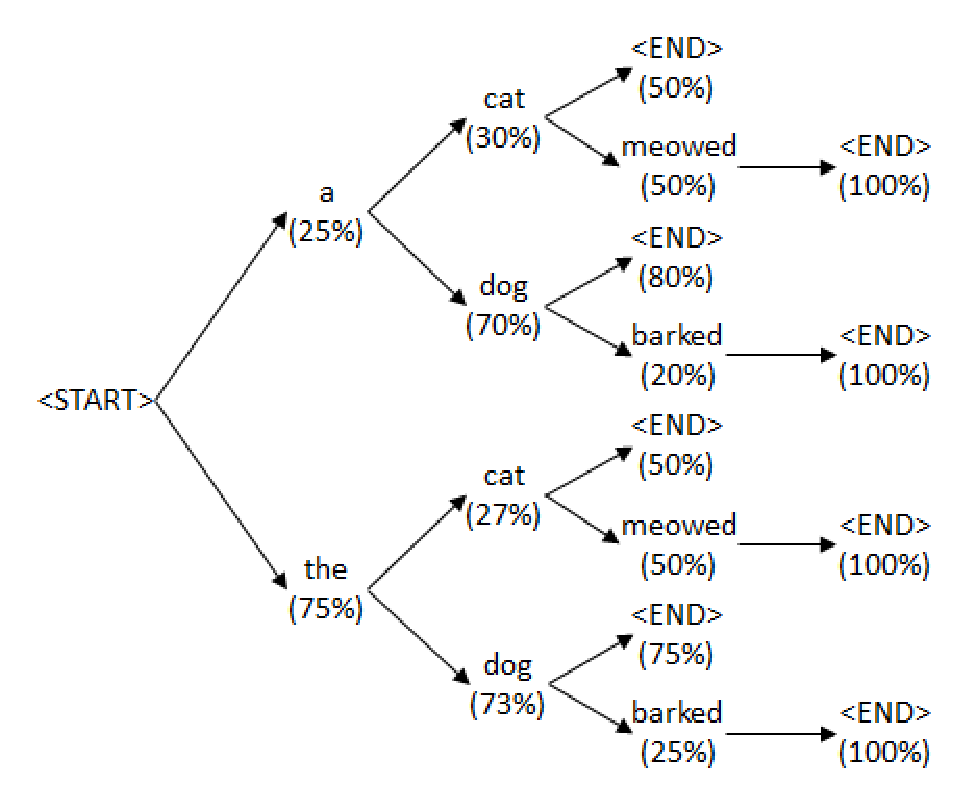
\includegraphics[width=0.6\textwidth]{figures/lm_tree.eps}
  \end{center}
\end{slide}

\begin{slide}[toc=Text generation]{Text generation}
  Using a language model, new texts in the language can be generated on the
  basis of the model's generative probability distribution.

  In terms of the tree structure shown on the previous slide, we are looking for
  branches on which the sum of weights (the log probabilities) are large.
  Exhaustive search is unfeasible, well-known strategies include
  \begin{itemize}
  \item greedy search,
  \item beam search, and
  \item stochaistic beam search.
  \end{itemize}
\end{slide}

\begin{slide}[toc=Evaluation]{Evaluation}
  Language model evaluation can be
  \begin{itemize}
  \item \emph{\gold extrinsic}: how well does the model do as a component in a
    spell checker, speech-to-text system etc., or
  \item \emph{\gold intrinsic}: how well the assigned probabilities correspond
    to the texts in a test corpus?
  \end{itemize}
  The most widely used intrinsic evaluation metric is \emph{\gold perplexity} on
  a corpus. A language model $\mathcal M$'s perplexity over the sequence
  $\mathbf w = \langle w_1,\dots, w_n\rangle$ is
$$\mathbf{PP}_{\mathcal M}(\mathbf w) = \sqrt[n]{\frac{1}{P_{\mathcal M}(\mathbf w)}}.$$
\end{slide}

\begin{slide}[toc=]{Evaluation cont.}
  With the chain rule perplexity can be rewritten as

$${\sqrt[n]{\frac{1}{P_{\mathcal M}(w_1)}\cdot \frac{1}{P_{\mathcal M}(w_2 \vert w_1 )}\dots\cdot \frac{1}{P_{\mathcal M}(w_n\vert w_1,\dots, w_{n-1})}}}$$

which is exactly the \emph{geometric mean} of the reciprocals of the conditional
probabilities of all words in the corpus.\bigskip

In other, words, perplexity measures, ``how surprising'', on average, words
(continuations) are in the corpus for the language model.
\end{slide}

\begin{slide}[toc=]{Evaluation cont.}
  Taking the logarithm of perplexity, with a few simple steps of algebraic
  manipulations we can see that the result is

  $$
  - \frac{1}{n} \left(\log P_{\mathcal M}(w_1) + \sum_{i=2}^n\log P_{\mathcal M}(w_i ~\vert~ w_1,\dots, w_{i-1})\right),
$$

which is the average cross-entropy and negative log-likelihood per word. A
simple consequence: by minimizing average cross-entropy or maximizing average
log-likelihood one also minimizes the model's perplexitiy on the training data.
\end{slide}

\section{N-gram based modeling}

\begin{slide}[toc=Estimating probabilities]{Estimating  probabilities}
  How can we estimate the required $P(\mathbf{w})$ probabilities from a corpus
  of texts? We could try to use occurrence counts:
  $$
  P(\mathbf{w}) \approx \frac{C(\mathbf{w})}{C(\mathrm{all~~texts~~in~~corpus})}
  $$
  but in any realistic corpus most texts occur only once and a lot of possible
  texts not at all. One option is switching to continuation probabilities: 
  
  $$
  P(w_{i} ~\vert~ w_1,\dots,w_{i-1})
  $$
\end{slide}

\begin{slide}[toc=]{Estimating  probabilities cont.}
  Using, again, count based estimation we could have
  $$
  P(w_{i} ~\vert~ w_1,\dots,w_{i-1}) \approx
  \frac{C(\langle w_1,\dots,w_{i} \rangle)}{C(\langle w_1,\dots,w_{i-1} \rangle
    )}
  $$
  but with the same data sparsity problem. One way of alleviating it is to use
  the
  $$
  P(w_{i} ~\vert~ w_1,\dots,w_{i-1}) \approx P(w_{i} ~\vert~
  w_{i-k},\dots,w_{i-1})
  $$
  approximation for a certain $k$, using the assumption that the continuation
  probabilities are (approximately) determined by the previous last $k$ tokens
  in the sequence.
\end{slide}

\begin{slide}[toc=\emph{N}-grams]{\emph{N}-gram language models}
  Using this approximation, the probability of a $\langle w_1,\dots,w_n \rangle$
  sequence can be calculated as
  \begin{small}
  $$
  P(w_1) \prod_{i=2}^k P(w_{i} ~\vert~ w_{1},\dots,w_{i-1})  \prod_{i=k+1}^n P(w_{i} ~\vert~ w_{i-k},\dots,w_{i-1}),
  $$
\end{small}
and the big advantage is that the
  $$
  P(w_{i} ~\vert~ w_{i-k},\dots,w_{i-1}) \approx
\frac{C(\langle w_{i-k},\dots,w_{i}\rangle)}{C(\langle w_{i-k},\dots,w_{i-1} \rangle)}
  $$
  estimates can be based only on the counts of maximum $k+1$ long subsequences
  in the corpus, so called $N$-grams ($N=1, 2, 3,\dots$).
\end{slide}

\begin{slide}[toc=Unigram models]{Unigram models}
  The simplest $N$-gram language models are \emph{\gold unigram} models,
  assigning to a sequence $\langle w_1,\dots,w_n \rangle$ the probability
  $$
  P(w_1)\cdot P(w_2)\cdot \dots \cdot P(w_{n-1})\cdot P(w_n)
  $$
  where the word probabilities can be estimated simply as
  $$
  P(w) \approx \frac{C(w)}{\sum_{w' \in V}C(w')}.
  $$
  Unigram models disregard the \emph{order} of words and the most probable
  sequences are simply those entirely composed from the most frequent word(s).
\end{slide}

\begin{slide}[toc=Bigram models]{Bigram models}
  Naturally, $N$-gram models based on longer subsequences are more fine-grained,
  even so called \emph{bigram} models ($N=2$) calculating sequence probabilities
  simply as
  $$
  P(\langle w_1,\dots,w_n \rangle) = P(w_1)\prod_{i=2}^n P(w_i ~\vert~ w_{i-1}),
  $$
  with
  $$
  P(w_2~\vert~ w_1) \approx \frac{C(\langle w_1,w_2\rangle)}{C(w_1)}.
  $$
\end{slide}

\begin{slide}[toc=Markov models]{Markov language models}
  $N$-gram models, in effect, model language with probabilistic finite state
  machines (Markov models), in which the states correspond to $N-1$-grams with
  positive probability.\bigskip

  E.g., in the case of an $\mathcal M$ bigram model, the states correspond to
  the vocabulary plus a start and end state, and the transition probabilities
  between states $w_1$ and $w_2$ are simply the $P(w_2 ~\vert~ w_1)$
  continuation probabilities.\bigskip

  It is easy to see that the $P_\mathcal{M}(\mathbf{w})$ probability of a token
  sequence $\mathbf{w}=\langle w_1,\dots,w_n \rangle$ is exactly the
  probability of the Markov model going through the states
  $\langle \textsc{start}\rangle,w_1,\dots,w_n,\langle\textsc{end}\rangle$.
\end{slide}

\begin{slide}[toc=]{Markov language models cont.}
  A very simple Markov language model:
  \begin{center}
    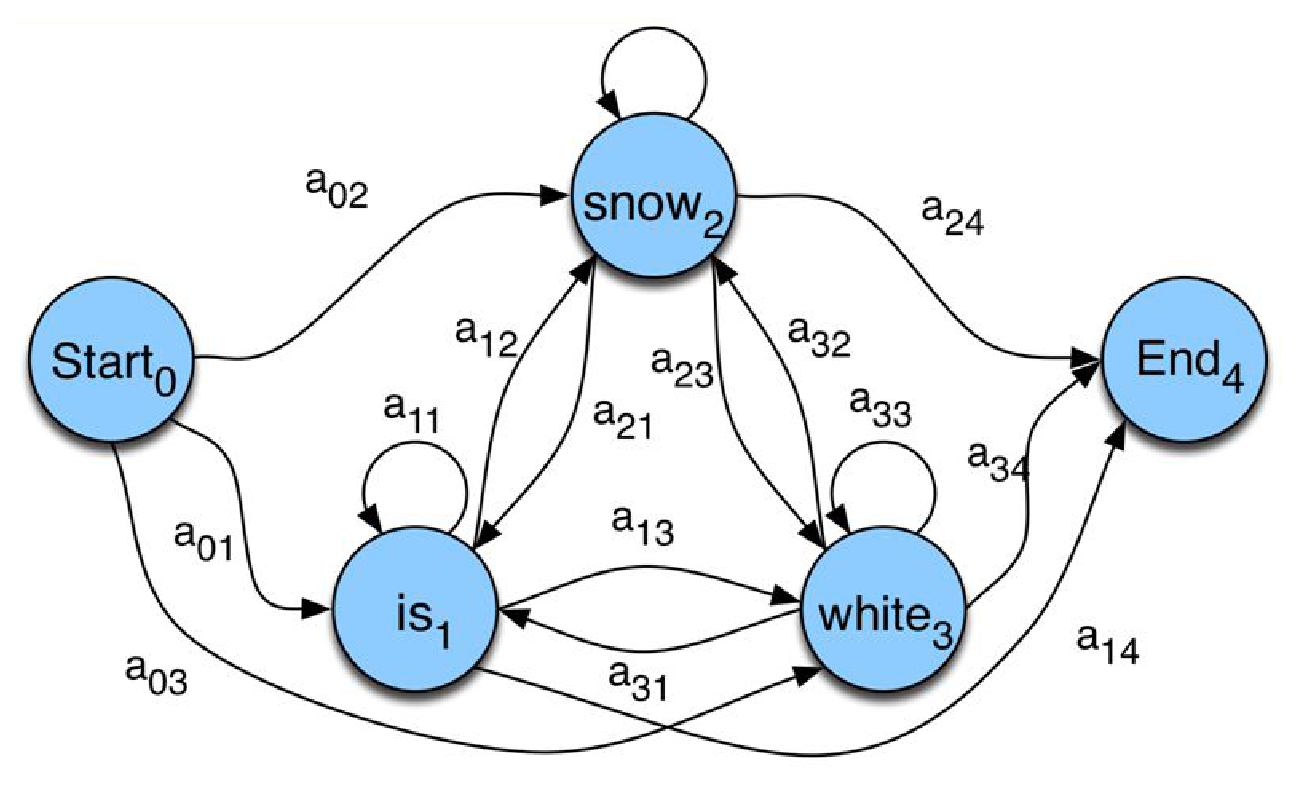
\includegraphics[width=0.9\textwidth]{figures/markov_lm.eps}
  \end{center}
  \small(Figure from D. Jurafsky's \href{https://slideplayer.com/slide/4578484/}{HMM slides})
\end{slide}

\begin{slide}[toc=Increasing \emph{N}]{Increasing \emph{N}}
  Since in reality human languages are way too complex to satisfy a low-order
  Markov assumption, $N$-gram models with higher $N$s (with $N=3,4$ or even $5$)
  typically have better intrinsic and extrinsic performance.
  Unfortunately, the number of linguistically possible $N$-grams grows
  dramatically with $N$. E.g., in the 1,024,908,267,229 token
  \href{https://catalog.ldc.upenn.edu/LDC2006T13}{$N$-gram corpus of Google} the
  $N$-gram counts are:
  \begin{itemize}
  \item unigrams: 13,588,391
  \item bigrams: 314,843,401
  \item trigrams: 977,069,902
  \item fourgrams: 1,313,818,354
  \item fivegram: 1,176,470,663.
  \end{itemize}
\end{slide}

\begin{slide}[toc=]{Increasing \emph{N}}
  The extremely high number of linguistically possible $N$-grams for higher $N$
  values poses two important problems:
  \begin{itemize}
  \item \emph{data sparsity}: a lot of possible combinations will not occur even
    in large text corpora, or occur only very rarely, so it's difficult to
    estimate their probability;
  \item \emph{model size}: even if estimates are correct, the model size will be
    enormous.
  \end{itemize}
\end{slide}

\section{Smoothing}

\end{document}



%%% Local Variables:
%%% mode: latex
%%% TeX-master: t
%%% End:

% LocalWords:  Tokenization
